\section{Durchführung}
\subsection{Versuchsaufbau}
Der Aufbau des Versuchs kann anhand des Fotos in Abb.\ref{fotosaufbau1} nachvollzogen werden.

\begin{figure}[H]
  \centering
  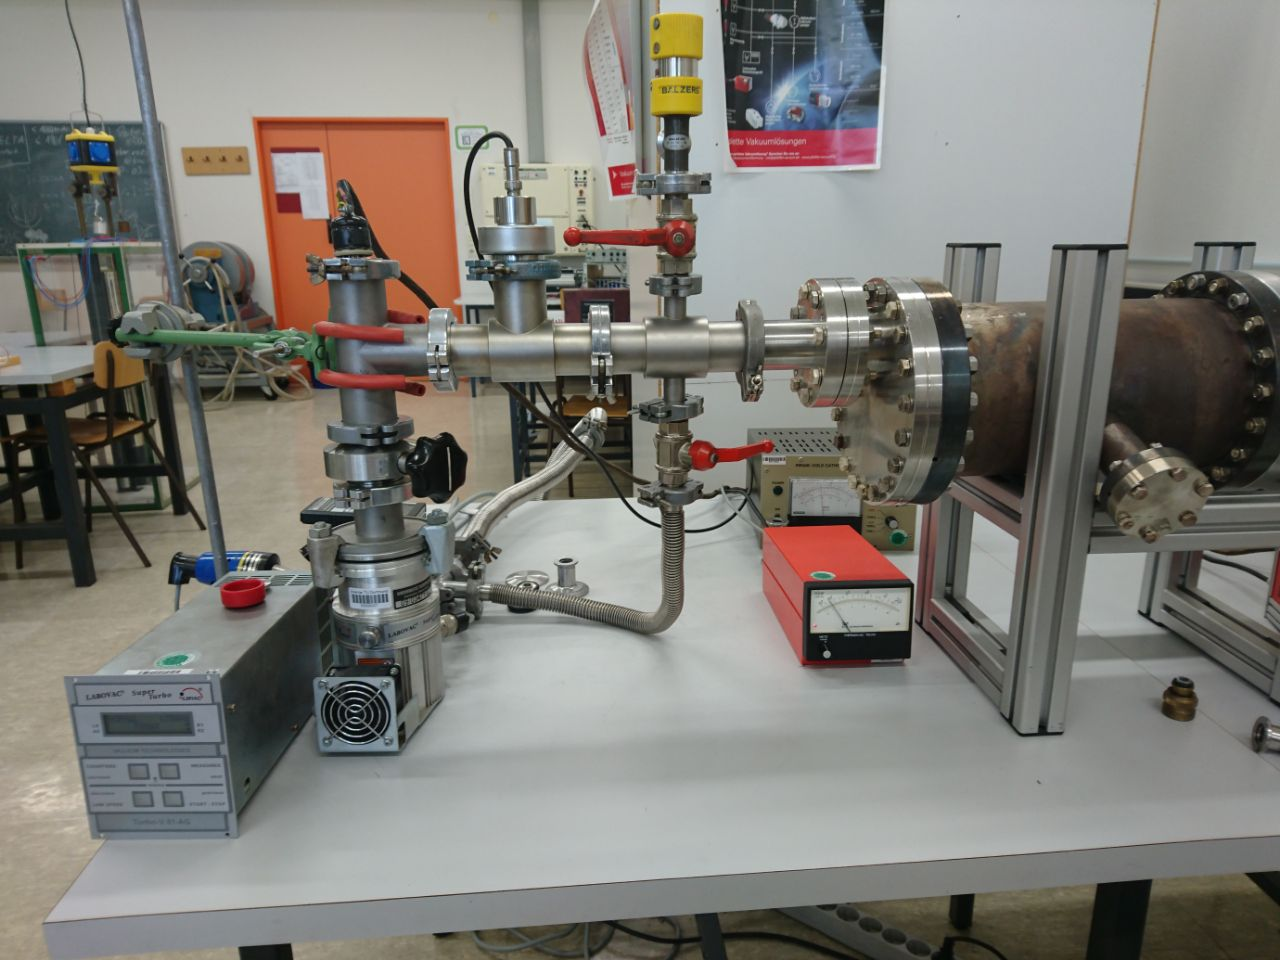
\includegraphics[scale=0.2]{Bilder/Versuch2.jpg}
  \caption{Frontansicht des Versuchaufbaus.}
  \label{fotosaufbau1}
\end{figure}
Zur besseren Übersicht befindet sich des Weiteren ein schematischer Aufbau des Versuchs in Abbildung $\ref{aufbauschema}$.
\begin{figure}[H]
  \centering
  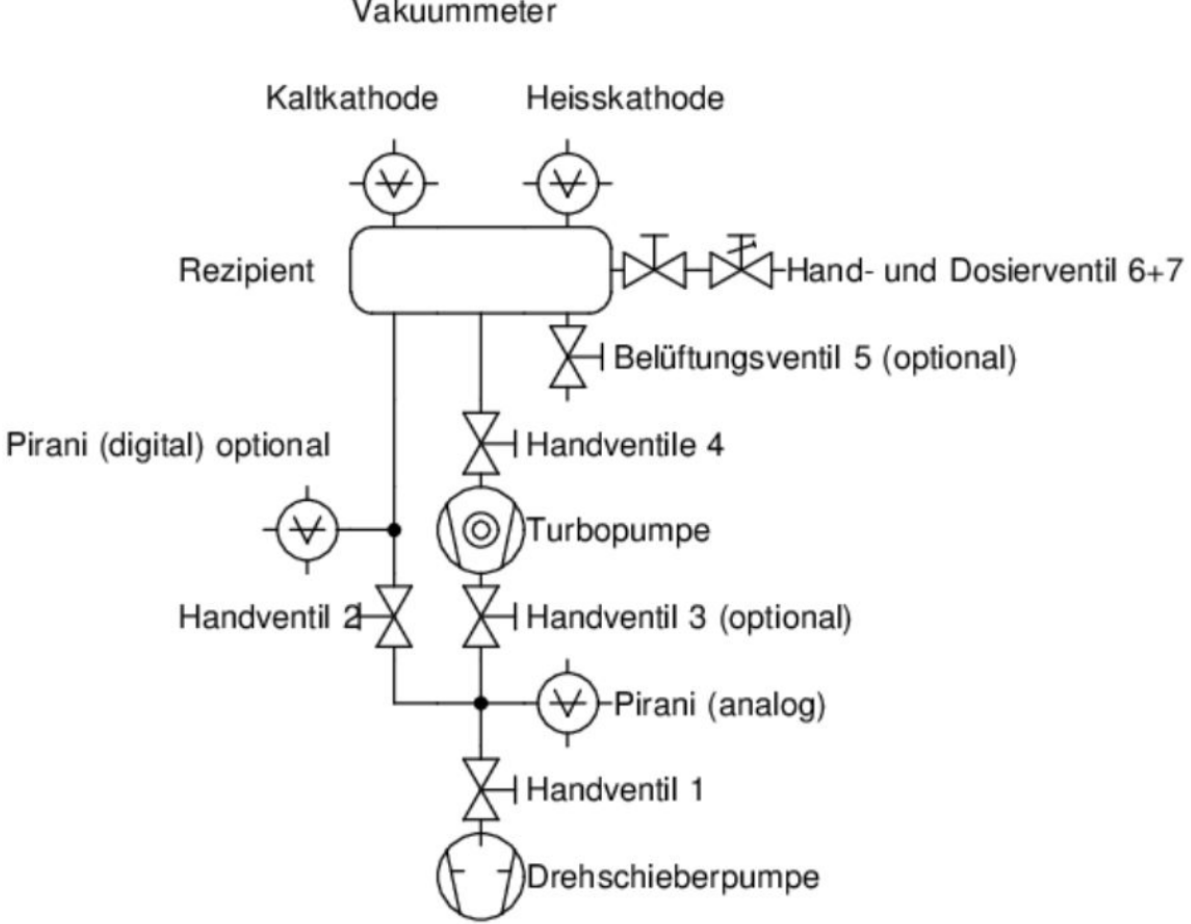
\includegraphics[scale=0.4]{Bilder/schemaVersuch.png}
  \caption{Schematische Darstellung des Versuchsaufbaus.\cite{anleitung}}
  \label{aufbauschema}
\end{figure}
